\setchapterpreamble[u]{\margintoc}
\chapter{Findings: Analytics in Use}

This chapter presents the research findings based on two of the six perspectives: \uuse and \iuse, \emph{i.e.} how app developers currently use mobile analytics and ways the use could be improved. 

\begin{figure}
    \centering
    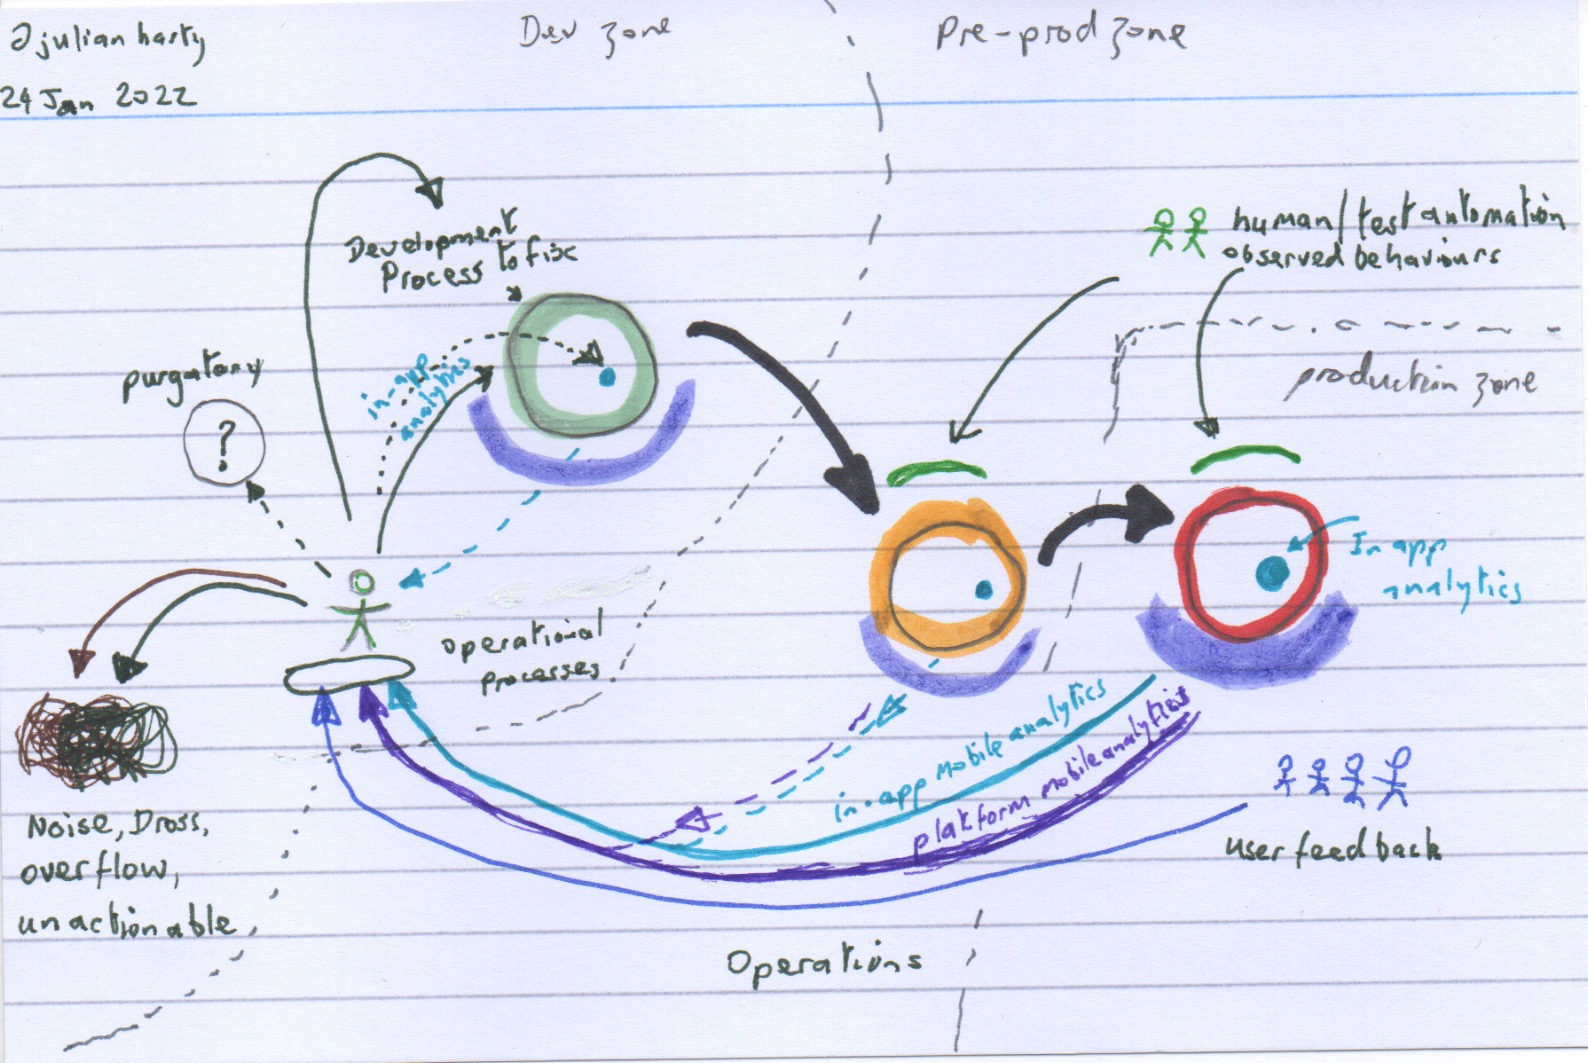
\includegraphics[width=\linewidth]{images/rough-sketches/dev-practices-with-mobile-analytics-24-jan-2022.jpeg}
    \caption{Dev Practices with Mobile Analytics}
    \label{fig:dev-practices-with-mobile-analytics}
\end{figure}

Figure \ref{fig:dev-practices-with-mobile-analytics} provides a conceptual representation of how analytics information flows are situated in the context of the development practices and artefacts. % ~\footnote{This figure will be revised pre-submission and keyed into the contents of this chapter. Versions of this figure may feature throughout the thesis with the pertinent elements highlighted and less relevant elements diminished or hidden from view.}. 
It builds on the concept of \secref{ptg-control-find-fix-zones-topic} with a focus on information sources, flows, and ways the information may be used.

At the highest level, the development context is organised into three zones: dev, pre-production, and production. Developers are in the dev zone where they work on tasks and create release candidates of their mobile app(s). The release candidates associated with each of these zones are illustrated by a coloured circle and their role, together with the relevant mobile analytics information flows, can be described as follows: 
    \begin{itemize}
    \item Green are releases in the safe zone, within the development zone. These are easy to work with and easy to cease.
    \item Amber releases are in the pre-release zone, they may be used by people external to the development team \textit{e.g.} colleagues, senior managers, closed, and/or open groups of users. The releases require some additional management to control the release rollout, some additional support, and they're harder to cease \textit{i.e.} to stop them from being used. App stores and/or third-party services may help make the releases available to these users.
    \item Red releases are in the production zone, they can be used by anyone who downloads them from the app store. Once releases reach production they can be extremely hard to cease entirely. In practice users are found who use years-old releases even after any mechanisms have been enabled to prevent those releases from functioning. 
    \end{itemize}

Within each release candidate developers can choose to incorporate one or more in-app mobile analytics libraries as part of a mobile analytics SDK. In the diagram the in-app mobile analytics libraries are represented by a small aquamarine spot. As the release candidate moves from development to pre-production usage is likely to increase somewhat, and as the release candidate is promoted into production the usage increases significantly, often by orders of magnitude for popular apps. The purple arcs under the circles represent the feedback being generated by the usage of that release of the app.


\begin{figure*}
    \centering
    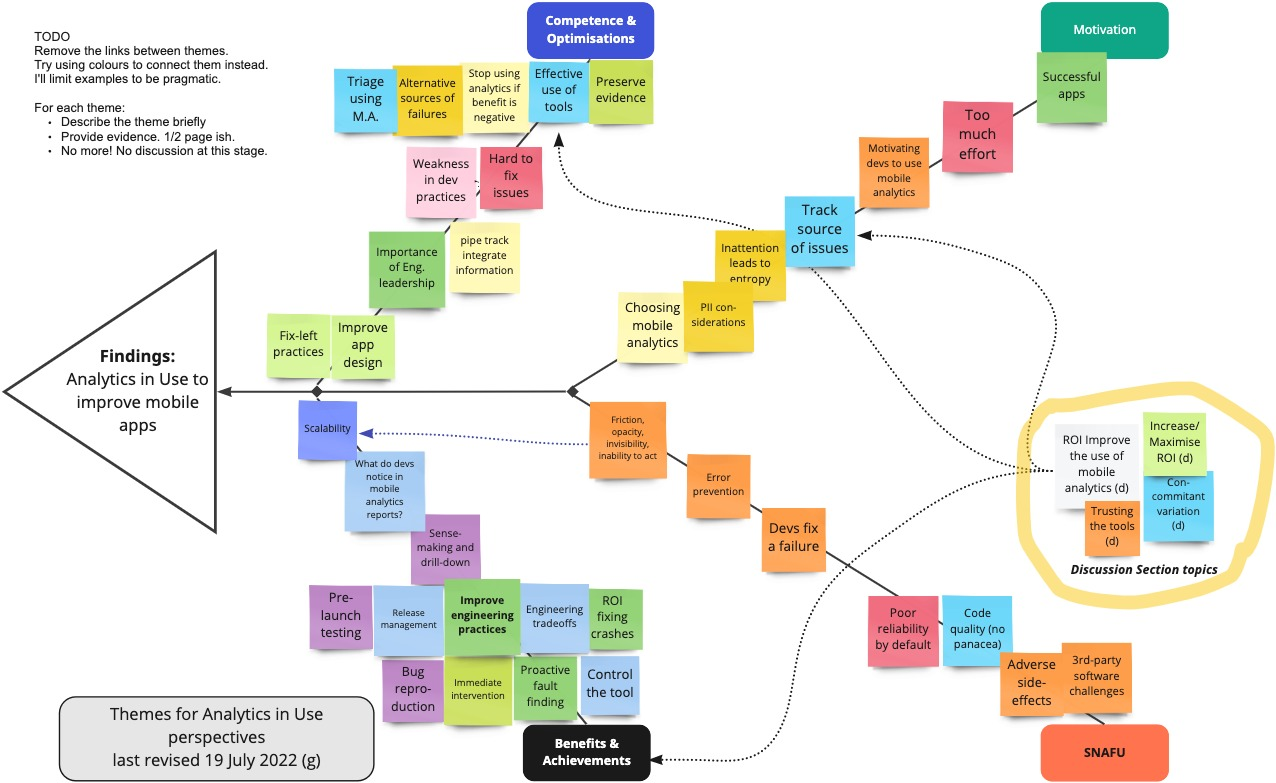
\includegraphics[width=\linewidth]{images/rough-sketches/analytics-in-use-fishbone-diagram-19-jul-2022g.jpeg}
    \caption[Analytics-in-Use fishbone diagram]{Analytics-in-Use fishbone diagram\\Source:~\href{https://miro.com/app/board/uXjVOlelPDU=/?share_link_id=219460632025}{MIRO board diagram}.}
    \label{fig:analytics-in-use-fishbone-diagram}
\end{figure*}

In the analysis of the findings there were 41 L1 themes identified in the spreadsheet. These were grouped into  4 L2 themes, they were also ranked to help select the most relevant examples for this chapter. Figure \ref{fig:analytics-in-use-fishbone-diagram} shows the mapping and key relationships between the themes.

The four level 2 themes are each covered in this chapter, they are: 1) motivation, 2) \Gls{snafu}, 3) competence \& optimisations, and 4) benefits \& achievements.

Motivation investigates what drives the developers to use mobile analytics to improve their apps, for instance is it `fire-fighting' or `optimisation'? \secref{aiu-motivating-factors-theme} presents evidence for this overall theme and the topic is discussed in the Discussion section of this chapter.

In terms of the higher-level themes, the context the developers are working in plays a major factor in what happens in terms of their use of mobile analytics so it's key to consider the evidence for this theme in \secref{aiu-snafu-and-real-world-conditions-theme}.

Benefits and achievements of using mobile analytics to improve their apps is discussed next to understand what they can accrue and what they can achieve. \secref{aiu-benefits-and-achievements-section} presents evidence for this overall theme.

And finally, competence and optimisation are vital factors in developers being able to obtain the benefits and gain the achievements. \secref{aiu-competence-and-optimisations-section} present evidence for this overall theme.

Before discussing the findings relating to improvements to the use of mobile analytics, the chapter also describes how interventions undertaken during the research increased the use of analytics by development teams.

\section{Motivating factors}~\label{aiu-motivating-factors-theme}
Motivation to use analytics spans a continuum from tactical behaviors to avoid and restrict failures, to strategic behaviours aimed at improving the design of the app and engineering practices of the team more generally.  In this section, we cover these motivating factors in turn, note: some examples extend beyond a single factor and some topics are grouped under a common heading. The \Gls{pii} topic will be covered in \secref{aiu-ethics-and-pii-topics}.

\subsection{Successful apps}\label{successful-apps-topic}
Developers and their organisations want their mobile apps to be successful. How success is determined can vary from one individual developer to another and from one organisation to another. Nonetheless unreliable apps are less likely to be considered a success by the developers or their organisation, which aligns well with the findings in this research.

\newthought{Improving app design:}%\todo{This is currently shown under Competence and Optimisations, decide where it fits best.} 
Another motivating factor of using mobile analytics is to improve the design of the app in terms of the user experience (UX). A more reliable and stable app is likely to improve the experience of users, this was a topic mentioned by several projects including \myindex{Moonpig}, \myindex{Moodspace}, and \myindex{SmartNavi}. It's not always easy to get the balance right in terms of informing users that the app contains mobile analytics - informing users may paradoxically reduce the user experience as illustrated by the \myindex{Pocket Code} app in the Discussion chapter in~\secref{discussion-empower-users}. At the time of the case study the Android app had pages of mandatory text presented to new users of the app.

\subsection{Motivating devs to use mobile analytics} As the \Gls{cto} of \myindex{LocalHalo} stated: \emph{``If you have lots of crashes you have zero chance of being promoted [by the app store].''}\sidenote{Informal conversations indicate being promoted can increase downloads by at least an order of magnitude; so promotion is highly prized by startups in particular who are keen to increase their user base.} % Be interesting to study the before and after for the winners of https://android-developers.googleblog.com/2022/07/google-play-indie-games-festival-finalists-revealed.html (from 3rd Sept 2022)
% See also top 10 in europe for Jimjum Studios https://youtu.be/6cKCFYzBuwY?t=96

The use of additional general purpose analytics is not confined to the commercial apps, the \Gls{gtaf} team explained how they had actively used mobile analytics to reduce the crash rate of their key apps and announced their intention to increase their use of mobile analytics in order to improve the user experience of their apps~\sidecite{gtafblog2021_gtaf_accomplishment_2020}. 

An interesting example from grey literature is the use of an error budget where the developers have 20\% of their time available to work on technical improvements. If the app's crash free rate is above 99.9\% the team can choose their work freely, however when the crash rate exceeds 0.1\% then the developers must spend their 20\% fixing the problem (described as the situation in the literature)~\sidecite{koutun2021_how_to_deal_with_tech_debt_at_the_scale_of_super_app}.


\newthought{Improving crash rate}: this motivation featured in the work of many of the app-centric case studies. For example, the \Gls{gtaf}\index{GTAF} project reported several of their Android apps had experienced high crash rates which had adversely affected the user experience. The project team have learned the importance of paying attention to crashes being reported by mobile analytics tools. \myindex{Kiwix} and \myindex{Catrobat} project leads also reported a desire to reduce the crash rates, in both these cases the crash rate for their key apps far exceeded the bad behaviour threshold of 1.09\%, specified by Google Play. 

In terms of the app-centric case studies only one of the interview-based studies - \Gls{gtaf} - explicitly explained they had periods of fixing high crash rates. Several of their Android apps had experienced high crash rates which had adversely affected the user experience. The project team have learned the importance of paying attention to crashes being reported by mobile analytics tools. They also realised the importance of addressing high crash rates. Accordingly, the development team used outputs from mobile analytics to identify the most frequent crashes they wanted to fix. In contrast, the majority of the rest of the interview-based studies were predominantly working to maintain good quality, to varying degrees based on their active and ongoing use of mobile analytics.


All of the action research-based app centric case studies were prompted by excessively high crash rates \emph{i.e.} they acknowledged they wanted/needed help both to tame the high crash rates and to improve the rates further on an ongoing basis.

For Kiwix, there was a pernicious, insidious increase in the crash rates for several of the most popular Android apps. The project leads particularly wanted to reduce the crash rates for the worst offenders in terms of the apps. Similarly the crash rate for \gls{glossary-pocket-code}\index{Pocket Code} far exceeded the bad behavior threshold, of 1.09\%, and despite the various recommended software development practices the project team had not been able to tame the excessive crash rate.

C1, the commercial case study's Android app had a user-base of millions however bouts of issues in several releases of the Android app meant the app had significantly exceeded the \gls{glossary-bad-behavior-threshold}, of 1.09\%. They needed to solve the tactical issues in parallel with improving the engineering practices to reduce the likelihood of similar bouts and to encourage ongoing and long-lasting improvements to the quality of their app and the service. 

\subsection{Choosing mobile analytics}~\label{aiu-choosing-mobile-analytics-topic}
The commercial app-centric case studies all incorporated general purpose usage analytics into their apps in addition to error reporting, \myindex{Firebase Analytics} was the most popular choice, which is congruent with Firebase Analytics being the dominant market leader~\sidecite{appbrain_firebase}. \myindex{LocalHalo} chose \myindex{Sentry}, in part as it integrated well with \myindex{React-Native}, the cross-platform development framework they used for their mobile app. The C1 project chose to include several mobile analytics SDKs in the app. \myindex{Microsoft App Center} was incorporated for crash and error reporting.

As mentioned previously, several projects including LocalHalo chose to use a separate mobile analytics service for business analytics. 

The choice of which mobile analytics tools to use is in some ways a recursive characteristic. Firstly, there is the choice of whether to include any analytics within the app at all - the Kiwix project team chose not to in order to maximise the protection of end users' privacy and minimise the potential for repressive authorities finding and then abusing usage-related data to penalise end users of Wikipedia and similar material. The rest of the app-centric case studies included at least one in-app mobile analytics SDK in their app.

Some of the projects, including \myindex{LocalHalo}, \myindex{GTAF}, and the Commercial project\index{C1}, choose to incorporate several mobile analytics SDKs in their apps. Their reasons differed, for example LocalHalo used Mixpanel for business analytics and Sentry for technology-related analytics including crash reporting. Greentech apps appears to let each app developer decide on which mobile analytics service to incorporate. The corporate projects reasons were multi-factoral and outside the scope of the research.

Choices of SDK may change over time: for example the Catrobat project chose to remove in-app analytics from their flagship Pocket Code app as the replacement for the Fabric Crashlytics\index{Crashlytics!Fabric} \Gls{sdk} - Firebase Crashlytics\index{Crashlytics!Firebase} also collected and combined \Gls{pii} data with the crash reporting. Like the \myindex{Kiwix} project team they wanted to err on protecting the privacy of their users (which includes many school-age children) and reduce their contributions to the already vast digital footprint owned by global tech superpowers.

Secondly, there is the choice of which source to use for which purposes. For instance both \myindex{Android Vitals} and the many crash reporting SDKs report on app crashes. All the projects who used in-app mobile analytics for crash reporting\index{Crash reporting} preferred to use that service to monitor the crashes in their app, even if some crashes aren't reported in that tool, for example those that occur as the app is starting up. Of the development teams who used in-app crash reporting Moonpig were unusual as they \emph{also} actively and frequently used Android Vitals to monitor crashes and other failures.

Thirdly, there are choices to be made in terms of what to record and when to do so in terms of in-app mobile analytics. Various in-app mobile analytics SDKs provide facilities for error reporting in addition to crash reporting. Broadly errors in this context are connected to caught and handled Java exceptions~\sidenote{For avoidance of doubt this includes \myindex{Kotlin} and other JVM languages, errors reported in frameworks such as React Native, and caught signals in C++ code.}. Some SDKs include API calls to provide trails of `\gls{glossary-breadcrumbs}' that lead up to an error or a crash~\footnote{For instance, see \href{https://www.bugsnag.com/blog/android-breadcrumbs-support}{www.bugsnag.com/blog/android-breadcrumbs-support}.}. None of the app-centric case studies mentioned actively using these breadcrumbs, however the reports Sentry generated for the LocalHalo app indicate the Sentry SDK generated automatic \gls{glossary-breadcrumbs}~\sidenote{\href{https://docs.sentry.io/platforms/react-native/enriching-events/breadcrumbs/}{docs.sentry.io/platforms/react-native/enriching-events/breadcrumbs/}} and these helped identify the server was no longer functioning correctly in late 2021. 

%%%% Sources include: 
%%%%%%% https://www.bugsnag.com/blog/error-handling-on-android-part-7 
%%%%%%% https://github.com/backtrace-labs/backtrace-android
%%%%%%% https://backtrace.io/
%%%%%%% https://saucelabs.com/platform/error-reporting (which also mentions triage)
%%%%%%% For breadcrumbs several are listed in https://www.google.com/search?q=breadcrumb+crash+reporting+android 

Caught exceptions, signals, etc. are not the only form of error that might be of interest to developers. Projects including \myindex{SmartNavi} and \myindex{Moonpig} used general purpose mobile analytics for reporting additional errors, for instance that affected the user experience. Similarly the general purpose mobile analytics and the crash reporting SDKs both collect contextual and runtime information and developers sometimes use this information.

\newthought{Too much effort:} Paradoxically, sometimes developers choose \emph{not} to apply the results of mobile analytics. Developers may perceive the effort required for something is too much and therefore take alternative action (including inaction). Examples from the case studies include developers choosing to ignore Android Vitals. Sometimes they do this as they've chosen to use another mobile analytics service that provides some of the information Android Vitals provides, particularly on crashes; an example is from \myindex{Moodspace}, where the \Gls{cto} noted: \emph{``ANR \& crashes: I usually use crashlytics, so never really use this tab. the reason being, that the play console used to be very unreliable for crashes.''} Others, \emph{e.g.} \Gls{gtaf}\index{GTAF} choose to ignore `hard to fix' issues, a topic discussed later in this chapter.

\newthought{Developer-controlled characteristics: }
Developers have a choice of how much to use a mobile analytics SDK, and similarly they can choose whether to have specific configurations for different environments, \emph{e.g.} for pre-production environments \emph{vs.} production. As illustrated in \sidecite{harty2021_logging_practices_with_mobile_analytics} 50 of 107 projects only used the minimal default initialisation rather than calling the rest of the Firebase Analytics API. None of the app-centric case studies relied on the minimal default initialisation, presumably by agreeing to participate in this research they were also motivated to use the SDK more extensively. 

In the commercial case study, \myindex{C1}, in pre-production release candidates used a distinct client-ID so the analytics outputs were separated from production traffic. The app was also configured to generate additional logging in pre-production builds.

\subsection{Ethics and Personally Identifiable Information (PII)}~\label{aiu-ethics-and-pii-topics}
The topic of \Gls{pii} has been mentioned several times already. A related topic is on the ethics of collecting mobile analytics data whatsoever, and if so, whether to default to opt-in or opt-out, and then in terms of what data gets collected, by whom, and for what purposes. 

As mentioned in \secref{aiu-choosing-mobile-analytics-topic} the \myindex{Kiwix} project chose not to incorporate any in-app mobile analytics or data collection for ethical reasons - to protect the privacy and provide safely for end users who might be heavily penalised for even using the Kiwix app and possibly imprisoned, or worse. In contrast the \myindex{Catrobat} project was initially keen to extend the use of in-app mobile analytics until they realised the type and amount of data collected by the mobile analytics SDK. 

\begin{kaobox}[frametitle=Comparisons with the `web']
In the related domain of websites and web apps similar there are challenges and legislation that pertains to the same topic in terms of the ethics of the collection of both cookie-related and other data.

The design and implementation of mobile apps has led to an app packaging any tracking or analytics within the \gls{glossary-app-binary} and although there are parallels with first and third party tracking, apps don't make that distinction for end-users, nor do they appear to have the need to ask users to accept `cookies' as the app doesn't actually use exactly the same mechanism for tracking.

In practice mobile apps appear to be `behind the curve' compared to web apps in terms of user consent. It might be at par in terms of how Google combines the analytics data from multiple apps using Firebase and/or Google Analytics embedded in apps, an assessment of changes Google made to web-based data collection is described in \sidecite{anon2018_google_stealthily_enables_super_profiles}.
% See also https://archive.epic.org/privacy/doubletrouble/ for a historical perspective from around 2000. and
% 106-2 Hearing: Online Profiling and Privacy, S. Hrg. 106-1117, June 13, 2000 (in my misc folder, via Google Books' digitisation service. This discusses how DoubleClick 'works' back in 2000. Google acquired DoubleClick around 2007 (I was employed in unrelated areas of Google at the time). and (Case No COMP/M.4731 – Google/ DoubleClick) European case in 2008.
\end{kaobox}

Several of the development teams had to make explicit decisions whether to use mobile analytics and if so which one they would use. The \myindex{Kiwix} project team chose explicitly to exclude mobile analytics from their apps to reduce the potential for end users to be tracked and potentially imprisoned through their use of the app and Wikipedia content in particular~\sidenote{The Kiwix project was developed to provide offline access to all of Wikipedia (at the time it was far smaller than today). It was then extended to support and provide lots of other content and material, nonetheless Wikipedia content is most likely to put end users at risk in various jurisdictions.}.

The Kiwix team did decide to use the platform-provided analytics from Google Play Console on the grounds that if the end-user had a) installed the Kiwix app from Google Play and b) had enabled (or at least not disabled) Google's collection of usage and performance data from their phones then the users were not being compromised by the devs using the analytics generated from the data those phones and tablets had provided.

The Catrobat team started by adding Fabric Crashlytics into their Pocket Code Android app several years before becoming a case study for this research. After seeing the results of applying the techniques from this research they choose to add Crashlytics to their iOS Pocket Code app and were also planning to use Firebase Analytics to record more granular usage data to both the Android and iOS apps. However, as a side-effect of migrating from the Fabric Analysis to Firebase Analysis - using the same client side SDK release they discovered they started receiving demographic data in tandem to the reliability analytics. Google then set a deadline where developers would need to replace the Fabric client side SDK with a similar one from Firebase to continue receiving any of the reports. The Catrobat team decided to stop using Crashlytics entirely rather than having demographics meta data collected by these SDKs in their apps. The Catrobat team had no objections to continuing to use the platform-provided analytics.

\newthought{Impact of ethical decision to remove mobile analytics: } The Catrobat project team chose explicitly to remove support for Crashlytics in the Pocket Code app when Google's deadline for migrating to Firebase Crashlytics expired. At the time, the project team discussed whether to keep Google Analytics support in the Pocket Code app.  
\href{https://github.com/Catrobat/Catroid/pull/3832}{Pull Request 3832} in the Pocket Code repository provides a written record of the changes made to the codebase and the discussion.


\section{SNAFU and real-world conditions}~\label{aiu-snafu-and-real-world-conditions-theme}
Software development, including developing apps, takes place in the real-world where there are often multiple conflicting demands on the time of participants - the developers. Therefore, absolutes, superlatives, and other pure approaches are unlikely to work. Bugs will happen, automated tests, if written at all, won't necessarily test much or test in depth, \xcancel{bugs will happen}, nothing will be perfect.

The impracticality of perfection leads to real-world consequences, to coping strategies, to pragmatic behaviours, and so on. There's a term, \Gls{snafu}, Several examples of \Gls{snafu} emerged in terms of a) developing apps, b) in the development teams using mobile analytics, and c) an accidental misconfiguration pre-release that led to a mute release of \myindex{Pocket Code}.

Firstly, in terms of developing apps, there is \textbf{poor reliability}\index{Poor reliability!SNAFU} of the apps in use by default. \myindex{Kiwix}, \myindex{Catrobat}, \Gls{gtaf}\index{GTAF}, and the Commercial project, \myindex{C1}, all had ongoing periods where the reliability was excessively poor and beyond one or more of Google's Bad Behavior Thresholds~\sidecite{play_console_help_android_vitals_2019}. Indications from the evidence gathered is poor reliability accretes when developers do not actively monitor mobile analytics and address the more severe of the failures that are reported. Conversely when developers do address these failures the reliability of the subsequent release of the app generally increases - a topic discussed in the next chapter.

\newthought{Friction, opacity, inability to act: }\index{Friction, opacity, inability to act!SNAFU} 
Another \Gls{snafu} factor is when developers do not have access to mobile analytics outputs, or when they do have access but they are not able to use the outputs productively. Surprisingly, this was common. As access to the mobile analytics tools is restricted by default~\sidenote{At least access has been restricted for every tool and service that feature in this research.} someone has to grant access to the particular individual developer. For \myindex{LocalHalo} only the \Gls{cto} and the researcher had access to \myindex{Sentry}, it is not clear why the rest of the development team lacked access.

Especially for larger teams, and teams where participation is periodic, many team members are not granted access. Three of the app-centric case studies exemplify this: \myindex{Catrobat}, \myindex{Kiwix}, and the Commercial Project, \myindex{C1}. There were two exceptions where all the developers had access: \myindex{Moodspace} where the sole developer had access, as he was also the account owner, and all the developers at \myindex{Moonpig} are provided with at least read access to \myindex{Google Play Console} with Android Vitals and to \myindex{Firebase Analytics}.

The lack of access for team members increases the importance and value of populating bug reports with pertinent information from the mobile analytics report(s).

\newthought{Weaknesses in dev practices}\index{Weaknesses in dev practices!SNAFU}
The third example of \Gls{snafu} is for the \myindex{Pocket Code} project. An accidental misconfiguration during the release process led to the loss of Fabric Crashlytics data for that release. Fortunately, Google Play Console with \myindex{Android Vitals} continued to provide ongoing outputs indicating the benefits of having platform-level mobile analytics. The development team applied the correct configuration for the following release of the app and Fabrics Crashlytics data was restored for subsequent releases.

\subsection{Engineering tradeoffs}~\label{aiu-engineering-tradeoffs-topic}
Software developers have to deal with tradeoffs, for example between developing features versus improving the existing codebase. In terms of the stability and reliability of their apps there were various findings where engineering tradeoffs were made, for example the \myindex{Kiwix} project chose to substitute their very capable download manager for the basic functionality provided as part of Android~\sidenote{They subsequently replaced the Android-based code with an opensource download manager and that's overdue replacement at the time of writing.}

Another tradeoff made by the  \myindex{Kiwix} team was based on the perceived maintenance overhead of making interim releases of the app meant the dev leads rejected the proposal to make interim releases for various of the custom apps even though an interim release was likely to significantly improve the reliability of those apps \sidenote{Details in \href{https://github.com/kiwix/kiwix-android/issues/1426}{github.com/kiwix/kiwix-android/issues/1426}}. A secondary consideration was the burden of creating and rolling out releases of the custom apps; at the time the release process was burdensome for the developers. 

\myindex{Moonpig} took several months to first replace the third-party \myindex{Robospice} \Gls{sdk} and then deploy the new release without that library.\sidenote{Robospice is still in 500+ apps which may be experiencing an ever increasing crash rate as newer versions of Android become more prevalent, source \href{https://www.appbrain.com/stats/libraries/details/robospice/robospice}{www.appbrain.com/stats/libraries/details/robospice/robospice}.}
Release management is a key factor in decision making. Crash analytics helped quantify the effects on groups of affected users (those on newer releases of Android).

Flo Health have explicit tradeoffs between how developers spend their time developing their app. Firstly they only spend 80\% of the time on core development, the remaining 20\% is ring-fenced for other development work. This 20\% is either spent on whatever the developers choose to work on, or on addressing errors if any error budget has been exceeded~\sidecite{koutun2021_how_to_deal_with_tech_debt_at_the_scale_of_super_app}.


\newthought{Third-party software challenges}\index{Third-party software challenges!SNAFU}
%To include: Robospice, Chrome.apk, WebView exceptions, OkHttp.
Third-party software is not modified directly by the app's development team (there may be ways they can modify it in other ways however these ways are beyond the scope of this research). Therefore there may be challenges when the app developers want or need changes to the third-party software. Furthermore the third-party may control what modifications are made to that software. Sometimes the app developers lack the context, wherewithal, permission, and so on to effect timely changes to the third party software i.e. there may be third party software challenges.

In terms of using mobile analytics a couple of examples from the Kiwix case study illustrate some of the challenges app developers need to consider with third-party software that's virtually part of Android: the closely-coupled Google Chrome browser and the \Gls{glossary-webview}\index{WebView} component that provides many apps with an embedded web browser and has over 5 billion downloads~\sidecite{android_webview_app_2022}. Crashes have been frequently reported with both these components for the Kiwix apps amongst many others~\sidenote{For example even Google's GMail app, Facebook's app, and the BBC apps were adversely affected in March 2021 \cite{bbcnews2021_google_fixes_crashing_android_app_issues}.}. For some of the crashes the developers are able to change the source code of the app to address some of the crashes however many seem beyond the immediate control of the app developers \emph{and yet the crashes are counted by Android Vitals and Google Play Console towards the cumulative} `bad behavior threshold'. 

The Commercial project, like many, used the third-party opensource \myindex{okHttp} library which is in over 6\% of top apps and 5\% of all apps measured by AppBrain~\sidecite{appbrain2022_ok_http_stats}.
%
To the okHttp's project's credit they provide various automated tests which can help both developers of okHttp and users (i.e. developers) of software that incorporates okHttp in their apps and other software. As the feature set of okHttp increases so can the complexity of using these various features, as the commercial project discovered when a developer inadvertently made changes to improve logging that led to the crash rate increasing several fold. A key challenge for the team was both finding a fix and then testing the fix was effective \emph{before} the revised app was released in the app store (rather than waiting for mobile analytics to report any change in the measured failure rate). They did so with the benefit of building on parts of the existing opensource okHttp codebase.

Grey data sources are frequently used by app developers to discuss problems with third-party components with the two main homes for these discussions being \gls{glossary-github}\index{GitHub} projects and StackOverflow.com.

% x-reference research papers on developers' practices updating Android third-party libraries.
% huang2019_up_to_crash_3rdparty_libraries_on_android
% not_yet_cited_zhan2021_research_on_thirdparty_libraries_in_android_apps_an_SLR_etc
% salza2018_do_devs_update_third_party_libraries_in_mobile_apps
% polese2022_adoption_of_third_party_libraries_a_case_study_on_opensource_android_apps
%\cite{salza2018_do_devs_update_third_party_libraries_in_mobile_apps, salza2020_third_party_libraries_in_mobile_apps}

\newthought{Release management}
Two examples of release management have already been mentioned (for \myindex{Kiwix} custom apps and for \myindex{Moonpig}, both in \secref{aiu-engineering-tradeoffs-topic}), the Commercial Project also placed great importance on scheduling releases with the intention of maintaining the goodwill and encouraging adoption of the new release. 

Google Play Console incorporates various aspects of its reports including various pre-filtered reports from Android Vitals into a Release Management section of the online GUI. The Release Management also includes mechanisms to perform a Staged Rollout which is particularly pertinent for apps with large userbases where it helps the development team to obtain focused information about the reliability and the adoption of the new release while also constraining the risk of a release failing in production~\sidenote{An overview of the Release Management features launched in Summer 2020 are covered in a short video \href{https://www.youtube.com/watch?v=vyReHI1eSSU}{www.youtube.com/watch?v=vyReHI1eSSU}.}. 

The product owners for the Commercial Project learned about how to combine the Release Management reports (including Android Vitals aspects in particular) and Microsoft App Center's reports in order to have greater insights into the vital signs and overall health of new releases. Android Vitals was seen to provide fast feedback into the health of a series of releases of the Android app and it was a highly effective early warning indicator of reliability issues emerging in a new release. Of note, staged rollouts cannot be reduced, nor can staged rollouts be targeted to users of a particular release of the app, so it's not currently practical to perform incisive upgrades to replace a failing release without also upgrading some portion of the other users of the app.

\subsection{Sense-making and decision-taking by developers}~\label{aiu-sensemaking-and-decision-taking-by-developers-section}
Beacon-finding and drill-down parallel similar practices used by app developers when they use mobile analytics as inputs to their development work and as feedback for [their] previous development work. One example is from \myindex{Moonpig} where they identified the pattern connecting the crash rates and Android versions related to the \myindex{RoboSpice} library that was being used in the Moonpig Android app. The RoboSpice GitHub project confirmed the factors that led to the increase in the crash rate which were caused by Android tightening the restrictions on background processing in order to save battery life. 

There are parallels between the sense-making process used by developers and those performed by end-users, described in \sidecite[][pp. 5:15-5:16]{grigoreanu2012_end_user_debugging_strategies_a_sensemaking_perspective}, where developers forage for information in locations that are likely to contain answers (\emph{e.g.} on StackOverflow and on GitHub).

\begin{figure}
    \centering
    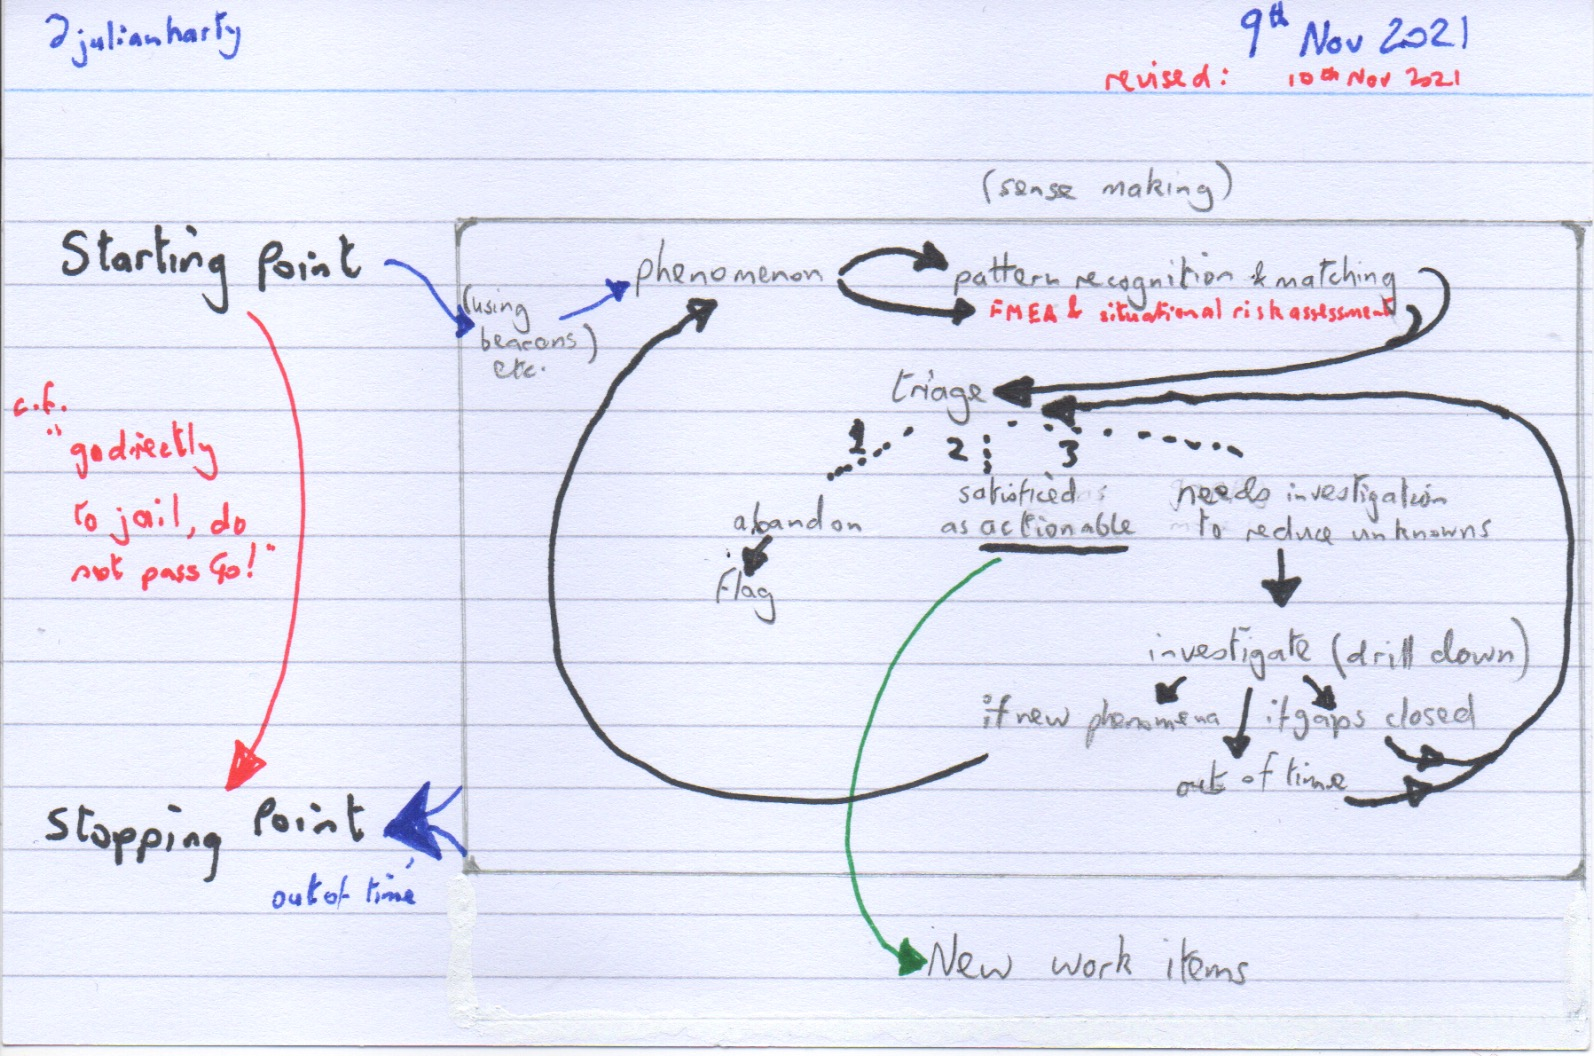
\includegraphics[width=\linewidth]{images/rough-sketches/practical-sense-making-process-10-nov-2021.jpeg}
    \caption{Sense-making process when development teams apply mobile analytics}
    \label{fig:practical-sense-making-process-when-dev-teams-apply-mobile-analytics}
\end{figure}


Figure~\ref{fig:practical-sense-making-process-when-dev-teams-apply-mobile-analytics} illustrates the sense-making and triage process used by development teams which shares various similarities with sense-making from a research perspective. These similarities mean the researcher and the practitioner may also share similar practices in terms of their analysis of phenomena found in mobile analytics tools. The triage and drill-down may be repeated several times where there is sufficient potential value in performing further investigation.

Developers seem to have finite time and resources to address issues reported by mobile analytics, how finite depended on their project and circumstances. The finite nature means they are unlikely to process every issue, so at some point they will cease processing the remaining issues - this is the stopping point in the figure.

The impact of reported failures is combined with situational-risk-assessment as a part of the decision-making process performed by developers during triage; for instance to consider whether this reported issue is worth addressing in the current development cycle, (\emph{e.g.} in the current sprint for teams who use sprints for work planning. Developers have to consider multiple criteria including personal, project, and product implications of making code and/or operational changes. From the same \myindex{Moonpig} example, the developers addressed high failure rate by replacing the \myindex{RoboSpice} library in the app relatively quickly, however they then choose not to make an interim, early, release as the crashes were tolerable. Conversely, the \myindex{Kiwix} team decided to make an immediate release with two bug fixes as the fixes had the potential to reduce the crash rate by about a third with minimal risk of introducing new issues. 

In contrast \Gls{gtaf}\index{GTAF} developers reviewed the various crashes and choose to work on the ones that they believed they could address quickly and effectively. Their criteria for the triage differed materially from the ones \myindex{Moonpig} used.

An untested hypothesis for their approach is introduced in the discussion chapter on page \pageref{discussion-decision-making-by-dev-teams-section}.

\subsection{Sources of suboptimal practices}
A cluster of several related themes: weaknesses in dev practices, premature satisfaction, what developers notice, and flaws in the mobile analytics may all lead to suboptimal practices.

\newthought{Weaknesses in dev practices}
Weaknesses in dev practices result in failure to address reliability issues. And where practices depend on one individual they can fail when the bus factor strikes. 

\newthought{Premature satisfaction}
A possible suggestion, an inference, is that many of the developers were often satisficed with what the mobile analytics tools reported - where they accepted local optima (determined through a combination of observation and asking the app devs), \textit{e.g.} they accepted the `top' crash cluster as the worst one. Therefore, if there are flaws in what is being reported the effects of those flaws may permeate into the results of what the developers \textit{do} and \textit{don't} do.

\newthought{Flaws in mobile analytics}
Indeed, as shown in~\secref{tata-flaws-topic} there are flaws in the groupings of similar failures in at least three of the mobile analytics crash reporting outputs.

\newthought{What developers notice}
One of the success factors is what the developers notice in mobile analytics reports (and what they don't notice does not get acted on).


\section{Competence and optimisations}~\label{aiu-competence-and-optimisations-section}
At a high-level there are two key competences, to enable the app to use any of the in-app analytics, details and examples of how to do so are in \secref{aata-code-facing-topics}, and then to actually use the reports and apply the results. The rest of this section presents the other competencies identified in this research.

\subsection{Using issue databases and preserving information}~\label{aiu-using-issue-databases-and-preserving-information-topics}
The \Gls{gtaf}\index{GTAF} team create issues in their online issue database \href{https://gitlab.com/greentech/}{gitlab.com/greentech/} for crashes and include links to the source information in the respective mobile analytics tool. These links are a) only available to people who already have access to the mobile analytics account, and b) are ephemeral. There are several ways development teams can extend the useful life of the private and ephemeral contents. 

In the three action-research app-centric case studies screenshots of the contents of the reports were combined with extracts of various pertinent statistics, for instance the frequency of a particular crash cluster. These contents were added to issues in the issues database. The developers appreciated the additional information (together with an online link to the relevant report which helped them check for any updates while that report was still available) they said it helped them appreciate the magnitude of the problem which, in turn, helped motivate them to address the issue sooner. The data was generally collected manually and pasted manually when the issues were raised, in part as automating the preservation of the reports is beyond the remit of individual team members.

\newthought{Integrating mobile analytics into the practices of the team}
One of the app-centric case studies, Moonpig, demonstrated they actively guarded against entropy through frequent, ongoing checking of the various mobile analytics services they used. They had an assigned developer on duty who was expected to check these services during the working day and action any issues or anomalies they noticed.

\subsection{Engineering leadership}~\label{aiu-engineering-leadership-topic}
There were clear correlations between having engineering leadership\index{Engineering leadership} participating and/or supporting the use of mobile analytics and in the measured reliability of the respective apps. \myindex{Moonpig} had integrated the use of mobile analytics in both development and operational aspects of their business. \myindex{Kiwix} achieved manifold improvements and sustained them while the Android project had a professional app developer as the project lead. 

% For the Pocket Code app, there has been an intermittent focus on addressing the causes of failures being reported by the mobile analytics tools.
In contrast the improvements in \myindex{Pocket Code} petered out after the loss of the Product Owner, a PhD student. One of the main reasons given by the project leadership was the loss of the product owner who successfully completed his PhD and moved to a role in Industry. 


\subsection{Triage}~\label{aiu-triage-theme}
%\julian{Include decision making, adverse side effects (which feeds into snafu and real-world conditions).}

The Triage is where the developers decide what to do, if anything, with failure clusters being reported by mobile analytics. Several of the projects confirmed used mobile analytics as a source when the issues are triaged and the others \textit{probably} did so too even though it was not discussed explicitly.

Broadly the triage process results in one of four outcomes:
\begin{enumerate}
    \item Accepted issues: which the project team intend to address.
    \item Pending issues: where the project team need more information before being able to reach a triage decision.
    \item Explicitly rejected issues: those the developers actively chose not to action, for instance as those impractical to address. Note: Some mobile analytics tools provide a facility for developers to ignore or mute these issues.
    \item Implicitly rejected issues: for some projects this applies to the majority of the failures reported by the various mobile analytics tools.
\end{enumerate}

The triage process sometimes led to issues being raised in the respective issues database for at least some of the issues they chose to action, for example Catrobat reported them in JIRA, Greentech Apps use \Gls{glossary-gitlab}'s\index{GitLab} integrated issues database, Kiwix similarly use \gls{glossary-github}\index{GitHub} issues. Moonpig often raised issues, however sometimes instead they simply modified the code where they believed the fault was clear and the fix quick and easy to do. The commercial app used recorded them in their organisation-wide issues database. However, projects did not necessarily record every such actioned issue. 

\newthought{Triaging failures}
One of the tasks for developers is triaging failures reported by mobile analytics. 

\subsection{Hard to fix issues}
The \myindex{GTAF} team used a heuristic when deciding which crashes to fix. They chose to work on those perceived as relatively easy to fix and which affected many users. They provided examples of easier to fix exceptions: \myindex{NullPointerException}~\footnote{Helpfully discussed in \href{https://en.wikibooks.org/wiki/Java\_Programming/Preventing\_NullPointerException}{en.wikibooks.org/wiki/Java\_Programming/Preventing\_NullPointerException}.} and \myindex{IndexOutOfBoundsException}~\footnote{Discussed in \href{https://stackoverflow.com/a/40006381/340175}{stackoverflow.com/a/40006381/340175}} versus some they found harder to fix: \myindex{IllegalStateException}~\footnote{An example of an Android specific crash is discussed in~\href{https://stackoverflow.com/questions/55158930/illegalstateexception-caused-by-intent}{stackoverflow.com/questions/55158930/illegalstateexception-caused-by-intent}} and native crashes~\footnote{Useful Android documentation on diagnosing native crashes \href{https://source.android.com/devices/tech/debug/native-crash}{source.android.com/devices/tech/debug/native-crash}}.

\myindex{SmartNavi} found it was not practical to identify or try resolving several low-frequency crashes that were only reported for unfamiliar and unavailable devices in China. As there was a sole developer on a voluntary project there was little scope to invest significant time and resources.

\subsection{The fix process}~\label{aiu-the-fix-process-topic}
Fix processes for issues found from mobile analytics are similar to fixing issues found from other sources, for instance: from testers, from app store reviews, and so on. There are some particular nuances when mobile analytics is the source; for example, the mobile analytics report will generally include one or more instances of a stack trace together with precise meta information. Mobile analytics also includes analytics such as any patterns of the failure. \sidenote{As an aside, several development environments can directly process and help analyse a stack trace for an app, for example in Intellij (which also underpins Android Studio used by many Android developers) \href{https://www.jetbrains.com/help/idea/analyzing-external-stacktraces.html}{jetbrains.com/help/idea/analyzing-external-stacktraces.html}.}. 

The combination of failure details, meta information, and patterns can help the team prioritise, manage, and diagnose the bug more effectively compared to bugs from other sources. Also, mobile analytics can provide measurements of any improvements (and any degradations) of the updated app.

The teams varied in their how they fixed issues. Some fixed the source code directly without externalising the reproduction or testing aspects, others attempted to externalise one or more of bug identification, bug reproduction, and testing practices. Those who were working tactically seldom invested time to reproduce the failure or write automated tests, instead they relied on external sources to provide feedback \emph{e.g.} from testers and/or from mobile analytics reports for the new release.  

For the commercial app two of the developers invested the time to distill the cause of the crash to a minimum, reproducible example~\sidecite{stackoverflow2022_minimal_reproducible_example} written in pure Java (so the Android runtime was not needed, it complicates the runtime conditions and the tests run much more slowly as Android tests). A set of automated tests were created to reproduce the crash at will. The flawed code was then improved so it no longer crashed and performed all the intended actions (previously it crashed instead). The automated tests demonstrated the fix was complete and correct. All the source code was then integrated into the app's codebase (the tests continue to run directly in a Java Virtual Machine rather than needing an Android runtime so they could run quickly, doing so is a mature development practice by Android developers and not unique to this app or development team).


The fix process therefore generally includes: a) an assessment of any recognised patterns in the failure to help with bug management, and b) post-release monitoring of mobile analytics to see if the fix actually improved the measured reliability of the app in the new release that includes that fix~\sidenote{While it is possible for mobile apps to include in-app dynamic updates of code these are a) uncommon and b) discouraged by the app stores. Google Android has an API called in-app updates however it is more of a mechanism provided to enable app developers to write code that can query the app store for newer releases and for whether the user should be asked, encouraged, or required to perform an update %.
%- \emph{i.e.} not patches performed by the platform which are called in-app updates but aren't actually in-app updates to the code they are in-app processes that affect how the app behaves when an update is provided via the platform
\href{https://developer.android.com/guide/playcore/in-app-updates}{developer.android.com/guide/playcore/\hspace{3pt}in-app-updates}. In-app patches of the app binary are therefore outside the scope of this research.}. 

\newthought{Fixing crashes may be necessary but not sufficient}
One of the issues~\sidenote{\href{https://jira.catrob.at/browse/CATROID-379}{jira.catrob.at/browse/CATROID-379}} and associated bug fixes~\sidenote{\href{https://github.com/Catrobat/Catroid/pull/3362}{github.com/Catrobat/Catroid/pull/3362}} pertaining to the Pocket Code app and the hackathon\index{Hackathon}~\sidenote{Via \href{https://jira.catrob.at/browse/CATROID-405}{jira.catrob.at/browse/CATROID-405}} has a discussion written by one of the project leads in the Pull Request~\sidenote{\href{https://github.com/Catrobat/Catroid/pull/3362\#issuecomment-541055675}{github.com/Catrobat/Catroid/pull/ 3362\#issuecomment-541055675}}. 
He observes there are still issues where content is not downloaded however the app no longer crashes. The high crash rate was sufficient to motivate the developers to address the source of the crash in the source code, however more work was needed to fix the failures to download and apply content. In the Pull Request, the developers also discussed the ramifications of removing the visual indicators when the user triggers a download and decided to simply try to fix the crash. As the developers could not reproduce the crash they were not confident in their `fix' working.

\section{Integration}~\label{aiu-integration-section}
%\julian{Include pipelines, tracking the source of issues including re-visiting integration into the triage process, trusting the tools, ...}

Integration of the tools and systems in this context facilitates and improves the `working together' of mobile analytics with other software tools. It ranges from manual and often short term mechanisms to streamlined pipelining of mobile analytics outputs into other systems. Often there's a basic facility provided which enables issues to be raised directly from a mobile analytics web page.

The majority~\sidenote{Moodspace and LocalHalo did not provide any details of their bug tracking processes.} of the app-centric case studies partly integrated mobile analytics reports into their bug tracking process by storing at least some of the contents of the reports some of the time.  

Of the projects that recorded the failures found by mobile analytics, it appears the Catrobat project used the crash's stack trace without anything else of the crash cluster's details or analytics~\sidenote{Examples include: \href{https://jira.catrob.at/browse/CATROID-1025}{Issue CATROID-1025} and \href{https://jira.catrob.at/browse/CATROID-1030}{Issue CATROID-1030}.} Moonpig stated they recorded many of the failures however sometimes they short-circuited the bug tracking system and modified the source code directly where the likely fix was believed to be easy to address with minimal risk. As they monitored the various mobile analytics services assiduously post-release they had at least one safety-net, also they may have recorded pertinent information in their source code repository - as this was not available during the research it is impractical to check at this stage.

\myindex{Kiwix}, \myindex{Catrobat}, \myindex{LocalHalo}, only provided a subset of the development team access to the mobile analytics services. As a result, the rest of the team were blind to any reports or issues \emph{unless someone who has access provides the relevant information in the bug tracking system}. The \myindex{GTAF} project team record crashes reported by Firebase in their bug tracking system however they only embed the URL, they have not included copies of the pertinent details.

As can be observed in the Greentech project's issues database, for example, the developers include the URL that points to the pertinent report in the source mobile analytics service. These links work for a period, typically hours to weeks, and are limited to people who have access to both systems. They enable authorised users to quickly check the source material from the relevant issue. 

These links eventually decay once the source content is no longer available, as discussed in \secref{tata-integration-into-workflows-topic}. In the three main action research projects screenshots together with pertinent text-based extracts were included in the issues database to help preserve the information indefinitely. Similarly \myindex{Vitals Scraper} was developed and used to automate the collection of screenshots and the underlying data from Android Vitals to preserve the information and make it available for additional analysis.

\myindex{Microsoft App Center}, for example, has the facility where comments can be added to failure clusters. In the Commercial Project, \myindex{C1}, the developers sometimes added a key in the comment field to indicate this failure cluster was under investigation. The key was often a bug reference and the developers sometimes also included terse notes. Sadly, it was impractical to determine the criteria for the various behaviours by the developers as the team were working remotely, on another continent, and the commenting mechanism does not show who provided the comment, or when.

Despite best intentions on multiple projects there were examples where developers did not add the pertinent cross-referencing between the issues database and the mobile analytics service. %\pending{Ask Moonpig how they did the cross-referencing and how reliably/consistently it was done.}

At least one of the projects, the Commercial Project, used APIs provided by the mobile analytics service to systematically export the contents of the crashes and errors that were captured in that tool: Microsoft App Center~\sidenote{Note: several other mobile analytics tools also provide similar API integration points, some of these will be discussed in \secref{tata-integration-into-workflows-topic}.}. Doing so enabled the data to be mined in combination with various other sources of data, however the details are beyond the scope of this PhD.


\section{Benefits and achievements}~\label{aiu-benefits-and-achievements-section}
Development teams were able to benefit from using mobile analytics in various ways, \emph{e.g.} to improve their engineering practices, to respond and act sooner, and to perform proactive fault finding. By being informed through mobile analytics of the magnitude and scope of various failures they were able to work more effectively and take better control than when they did not have mobile analytics available to them. They were able to achieve more.

\subsection{Proactive fault finding}
\myindex{Moonpig} used Firebase Crashlytics and Google Analytics for diagnostics. They spent 30\% of time spent using Android Vitals to identify flaws and issues related to their Android app. %Examples of flaws that escaped into production, and when they were addressed. 
They noted, that while finding and fixing causes of crashes may be quick, the release may take several weeks before it's deployed.

In the commercial, \myindex{C1}, project the use of mobile analytics helped identify a major issue within days. The development of automated tests that reproduced the failure helped establish confidence in the tests and in the subsequent fix to the networking code. Proactive use of the \myindex{Release Management} reports in Google Play Console helped the team release the revised app with visibility into the effects of users updating and using the revised app. And, in general, proactive use of the release management reports helped the team make immediate interventions when there were indications of releases having adverse effects.

Note: in addition, training was provided to the Product Managers for the project on how they could use \myindex{Google Play Console}, \myindex{Android Vitals}, and the \myindex{Release Management} reports to provide them with direct visibility into the state of the app and indications on the effects on the end users e.g. through the installation and de-installation reports. This was one of the actions that helped scale the team's capabilities.

The majority of the app-centric case studies were known to use aspects of the \myindex{Release Management} tools in Google Play Console. The rest may also have done so, however, the information is not available from those case studies.


\subsection{Bug reproduction}~\label{aiu-bug-reproduction-topic}
Being able to reproduce bugs, ideally at-will, enables developers to work more effectively at addressing the bug and having confidence that their intended fixes actually do fix the bug. 
Bug reproduction can increase the developer's confidence the bug is real and can be managed, it is under control. Then they can make changes to the the software to determine whether their changes address (fix) the bug. 

The developers are not always able to reproduce bugs, for example the developers of the Pocket Code app had to apply their `fix' blindly with the immediate aim of fixing, \emph{i.e.} preventing, the crash \href{https://github.com/Catrobat/Catroid/pull/3362}{github.com/Catrobat/Catroid/pull/3362}.  In the commercial app, two experienced engineers spent several days in devising a consistent and clear way to reproduce a crash in the response handling and logging for proprietary code that interacted with the very popular OkHttp opensource library (more details are in the section on the fix process in Section~\ref{aiu-the-fix-process-topic}). This effort was deemed necessary and appropriate given the strategic importance of the app to the business and the effects of the crash on a significant subset of users' sessions.

The research also had mixed results reproducing bugs that were found and reported by mobile analytics.
%
The Kiwix project included crashes in several software components Google provides android developers: the \Gls{glossary-webview}\index{WebView} (an embedded browser), and \Gls{glossary-chrome-apk}\index{Chrome.apk} - the binary file for the Google Chrome Android app. It also included attempts to reproduce crashes in the app's codebase. 

\begin{itemize}
    \item One experiment used the same model of Samsung Android smartphone that incurred a higher than usual crash rate, however there was insufficient information available in Android Vitals to determine enough of the events that led to the crash or any of the contextual information. The manual interactive testing did not manage to reproduce the crash.
    \item Another experiment scripted the semi-autonomous Android Monkey testing utility where the script seeded each test run to make the sequence of generated inputs consistent with the aim of first triggering crashes and then having sufficient information to reproduce those crashes at will.
    \item Note: a third experiment was on hold for several years awaiting availability of the software tool, CrashScope. This became available in late 2021 and the testing is pending the configuration of the tests with the various apps.
\end{itemize}

With the exception of the Commercial project, none of the commercial projects (Moonpig, Moodspace, LocalHalo) provided examples of being able to reproduce crashes and other failures that were reported by mobile analytics; nonetheless they chose to use in-app analytics and the respective mobile analytics reports in preference to Android Vitals as they believed these tools provided more relevant reports with the necessary information to enable the developers to find and fix the causes of those crashes.

There are plenty of instances where app developers had to debug and try to fix failures without being able to confidently test the code to a) reproduce the failure, or b) evaluate the changes to the source code. Releasing the new version of the app and monitoring the effects became part of their practice, albeit some projects monitored more assiduously than others. This approach has parallels with the approach described in \sidecite{ghardallou2016debugging_without_testing} however they aim to prove relative correctness whereas using mobile analytics aims to measure characteristics of the software when in real-world use.

\subsection{Pre-launch reports}~\label{aiu-pre-launch-reports}
The \Gls{gtaf}\index{GTAF} project found crashes pre-launch through using - and paying attention - to the pre-launch reports. Many of the case-studies used pre-launch reports. 

\begin{figure*}
    \centering
    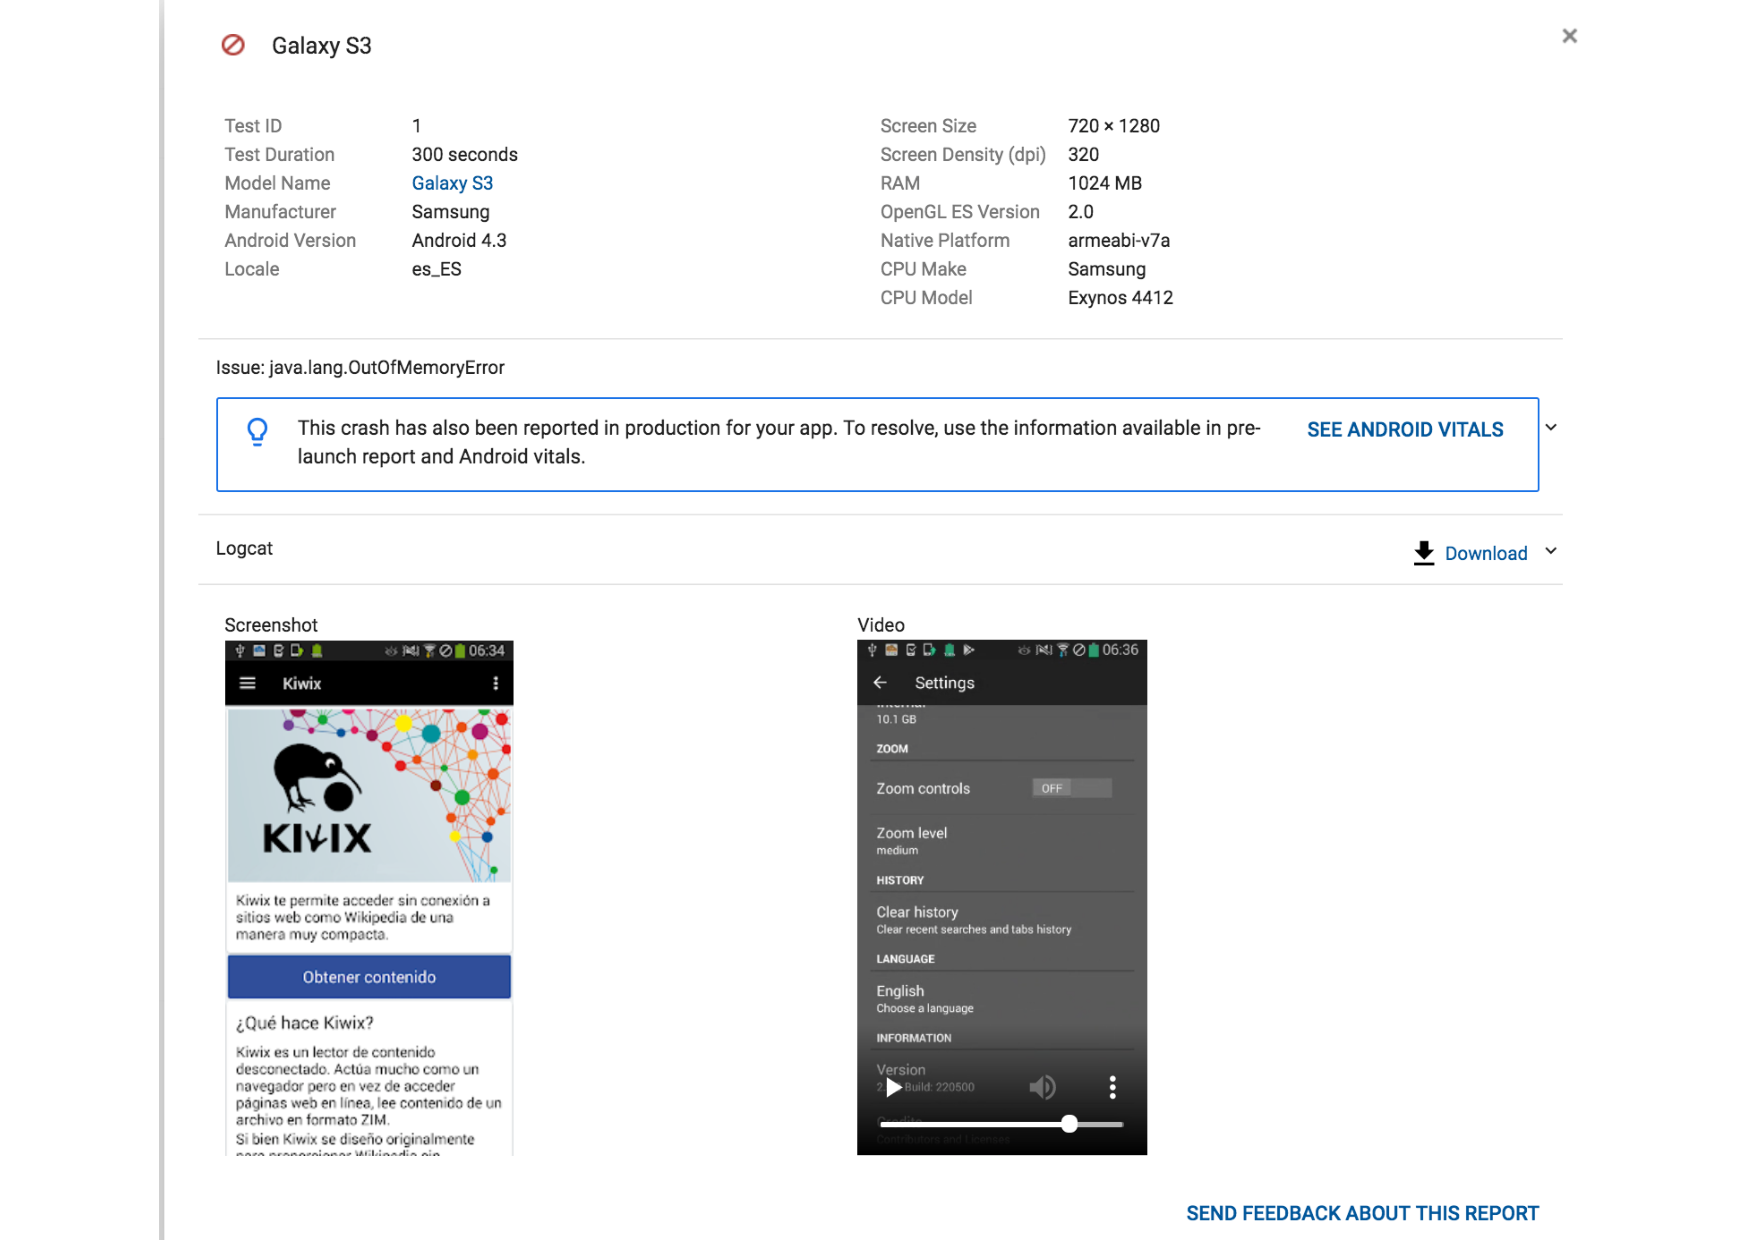
\includegraphics[width=\linewidth]{images/google-play-console/Pre-launch_report_Galaxy_S3_OOM_Exception_Details_(19-Jun-2019).pdf}
    \caption[Kiwix Version 2.5 \texttt{OutOfMemoryError} Exception]{Kiwix Version 2.5 OutOfMemoryError Exception, on 19-Jun-2019}
    \label{fig:pre-launch-report-kiwix-oom-also-in-production}
\end{figure*}

For the \myindex{Kiwix} Android app, the pre-launch report for a newer release (App version: 7230406.aab) showed results that indicated a degradation in the performance of the app compared to a previous release (App version: 7230405.aab). And a crash caused by a \texttt{java.lang.IllegalArgumentException Parameter specified as non-null is null: method org.kiwix.kiwixmobile.core.utils.LanguageUtils.getCurrentLocale, parameter context} occurred with a locale of `ar' (Arabic) on a Sony G8441 device, running Android 8.0.

A strength of the pre-launch reports is the automatic cross-referencing between crashes that were discovered during the pre-launch testing and those that occurred in that release subsequently in production. Figure \ref{fig:pre-launch-report-kiwix-oom-also-in-production} provides a good example, where a Java OutOfMemory (OOM) error was detected and a link to Android Vitals provided directly in the report. At that time the app had various memory leaks which the developers were identifying and addressing~\sidecite{kiwixandroid_issue_615_fix_memory_leaks}, and OOM errors occurred when testing the app on some low-end devices~\sidecite{kiwixandroid_issue_742_oom_running_espresso_tests}. The devs were using \myindex{LeakCanary}, an opensource tool designed to help Android developers identify memory leaks. 

Various developers have reported false positives \sidenote{\href{https://issuetracker.google.com/issues/160907013}{Could you fix Pre-launch report false-positives triggered by your own code base?}} and this error occurred in several of the case studies including \myindex{Kiwix} and \myindex{C1}. These false positives sometimes led to developers choosing not to use the pre-launch reports.

\subsection{Improving engineering practices}
\myindex{Moonpig}'s, engineering team used mobile analytics strategically and tactically to nip any unreliability issues `in the bud', \emph{i.e.} quickly and practically, in order to minimise adverse effects on the end users and the business. 

They incorporated \myindex{Firebase Analytics} for usage, crash, and  error reporting and they had developer's on rotation to monitor and triage any issues as soon as practical - within hours - after they arose in the mobile analytics reports. When unknown situations occurred the developers increased logging in the app (using Firebase Analytics as the conduit for the logging, similar to the use presented in \secref{section-sourcecode-analysis-to-augment-app-centric-case-studies}).


Conversely several of the case studies demonstrated that \textbf{inattention leads to entropy} in terms of using mobile analytics to maintain the stability and reliability of their apps. \myindex{Kiwix} lost the lead developer in early 2021 and first the crash rate and subsequently the \Gls{anr} rate increased markedly. \Gls{gtaf} similarly would experience bouts of excessively high crash rates until they focused their attention on addressing them. \myindex{LocalHalo} hadn't noticed the loss of reports in \myindex{Sentry} nor the increase in \myindex{Android Vitals} until the issues were pointed out to them via this research. None of the projects were immune from the adverse effects of inattention, however, \myindex{Moonpig} were by far the most effective at finding and addressing the issues quickly and their periods of inattention were brief.

Glspl(plr) can be incorporated into developer's practices to improve the quality of Android apps and several of the case studies, including \myindex{Kiwix}, \myindex{GTAF} and \myindex{Catrobat} use them. The reports are discussed in the Tools chapter, in \secref{tata-pre-launch-reports-topic}.


\section{Interventions to increase use of mobile analytics}~\label{aiu-interventions-theme}
\newthought{Research-led interventions}
Each of the three app-centric case studies that involved action research included one or more interventions. For the two opensource projects, Kiwix and Catrobat, hackathons\index{Hackathon} were used as they provided an immediate low-ceremony approach that enabled quick and effective collaboration. For the commercial project the intervention was performed over a period of approximately six months and involved working with several of the projects development team to help them understand how mobile analytics provides them with pertinent information and how to then apply that information to fix the underlying issues. 

\newthought{Project-led interventions}
% It might be worth relocating this to later in the thesis where we discuss pii and ethics.
For the Catrobat case study, the project leadership saw sufficient benefits from using mobile analytics after the hackathon\index{Hackathon} that they decided to also implement it in the iOS app. However, several months later they subsequently reverse this decision because of the data collection collected implicitly by Firebase Crashlytics. This topic is covered in \secref{aiu-ethics-and-pii-topics}.


\subsection{Mobile analytics in a larger context}
The research focuses on failures identified using mobile analytics and the processes where developers incorporate mobile analytics into those processes. There may be other sources of information about failures and there may be other causes of fixes and improvements.

\newthought{Crashes mentioned in user reviews: }
Mobile analytics is one source of information on failures, other sources may be available. In this research, many of the apps have reviews in the app store (Google Play) that mention crashes. The reviews vary in their specificity and the project teams seldom diagnosed the crash from the description in the review text.   

\begin{figure}
    \centering
    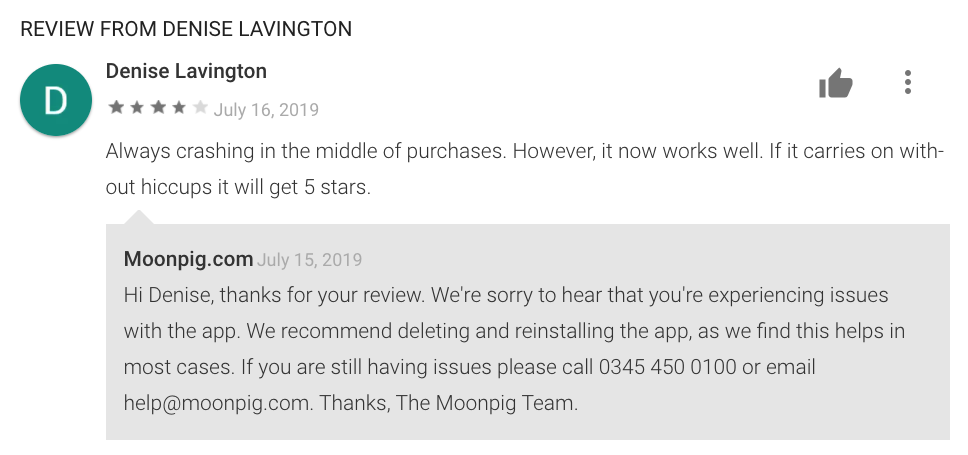
\includegraphics[width=\linewidth]{images/google-play/Denise-Lavington-Review-moonpig-crashing-2019.png}
    \caption[Moonpig: User Review in Google Play `Always crashes...']{Moonpig: User Review `Always crashing in the middle of purchases'}
    \label{fig:gp-review-denise-lavington-always-crashes}
\end{figure}

As a concrete example of perhaps the most detailed review, for the Moonpig Android app, on \nth{16} July 2019, Denise Lavington provided a review of the Android app and awarded the app four stars. The review said: \emph{``Always crashing in the middle of purchases. However, it now works well. If it carries on without hiccups it will get 5 stars."} Figure \ref{fig:gp-review-denise-lavington-always-crashes} shows the review in context in Google Play~\sidenote{The review is currently still available online (\href{https://play.google.com/store/apps/details?id=com.commonagency.moonpig.uk&reviewId=gp\%3AAOqpTOH68VB5eWqnu7UAqcC81_rbOfWl6dzL_g48jrg0T40MPWBkMxe01KjStXZF6F57nxZxQa-AqosRKDd1xQ}{here}) in Google Play, over two years after it was written.}.

The developer investigated this reported issue and could not find any crash in Firebase or Android Vitals that might affect purchases. A possible reason for why the crash did not appear in Android Vitals is that the underlying data is only provided by a user's device if they've opted-in to automatically providing their usage and diagnostics data~\sidecite{google_play_view_crashes_and_anr_errors} \textit{and} if the aggregate data exceeds an undocumented threshold (a topic discussed elsewhere in the thesis). 

Monitoring reviews can be useful to identify issues including user dissatisfaction (app reviews are discussed in the Literature, in \secref{rw-reviews-in-app-stores}). In this case there was insufficient evidence to corroborate the user's report. As a side note, Google Play Console provides automated analysis of reviews, including those that infer stability issues for instance that have the word `crash' in them~\sidecite{googlesupport_reviews_analysis}. In the author's experience the analysis is imperfect, future research might be of interest.

%%% Julian to continue here on 09 Sep 2022

\section{Improvements to the use of Mobile Analytics}~\label{aiu-itools}\index{\iuse}
\myindex{Moonpig} demonstrated a highly effective use of mobile analytics not only to detect failures, including \glspl{glossary-crash-cluster}, they also used mobile analytics to gain additional information of possible causes (similar to the concept of using \gls{glossary-breadcrumbs} however Moonpig used logging more holistically). The example from \myindex{C1} of devising automated tests to reproduce crashes that occurred in complex code and which required non-trivial work to implement suitable dynamic tests demonstrated that developers who are willing and able to invest the time can gain confidence in the reliability and behaviours of their software under realistic conditions.

As \myindex{Kiwix} demonstrated it is possible to increase the reliability for a failing app quickly and effectively. The next chapter includes a summary of the improvements in \secref{aata-improvements-in-crash-rates-topic}. In contrast improvements stalled for the \myindex{Pocket Code} Android app when the work was disrupted for various reasons in 2020.

Some improvements in use depend on the reporting and integration facilities offered by the tools, and similarly on the quality and timeliness of the reports, aspects of these are covered in \secref{discussion-empower-developers}, \secref{discussion-improving-mobile-analytics}. 

Others can be effected using the current services offered by the tools, for example relatively simple things such as enabling the entire team to use the mobile analytics, \secref{discussion-scalability}, through \secref{aiu-engineering-leadership-topic} that values mobile analytics and encourages using them on an ongoing basis, and by using them regularly, especially before release by using \acrfull{plr} and on release by using the \myindex{Release Management} reports. 

A pragmatic acceptance that an app will not be truly free of failures, means projects and teams should pick their own targets (these should be significantly higher than meeting the \gls{glossary-bad-behavior-threshold}\index{Bad behavior threshold}). \myindex{Android Vitals} provides quartiles per application category so a useful heuristic would be to be in the top quartile in terms of app stability.

As \myindex{SmartNavi} explained some failures are impractical to investigate or address, this was confirmed by the \myindex{Moonpig} case study:

\begin{quote}
    \emph{``I don't know why some crashes don't even show up but we honestly just accepted that Android is weird on some even weirder devices. As long as our crash-free rate is that high and will go even higher after the next update, we are happy.''} (source Moonpig developer)
\end{quote}


\section{Chapter summary}
This chapter presented ways mobile app developers used mobile analytics together with an overview of ways the use could be improved by app development teams. These findings are summarised below and discussed together with the other findings in \secref{chapter-dicussion}.

Motivations to use analytics included making apps more successful and usable, as well as consideration of ethical issues relating to collecting data from end users' devices. The processes associated with using analytics were also affected by the real-world conditions in which the development teams operates. For example, engineering choices made by the team can affect how analytics are used, as well as the techniques adopted by teams to make sense of analytics data. 

Additionally, this chapter identified a range of competencies used by development teams to make effective use of analytics, such as drawing on strong engineering leadership and ensuring effective information preservation using issue databases. 

Finally, it was possible to identify different types of benefits enjoyed by development teams as a result of using analytics. It was also noted that improvements in the use of analytics by the team depend on features supported by the analytics tools, including good reporting and integration capabilities. 

The features of analytics tools will be explored in chapter \secref{chapter-tools-and-their-artefacts}. Before this, the next chapter presents the effects of mobile analytics on apps and their artefacts.

